\subsection*{Threads Per Block}
We experimented with multiples of the warp size as the number of threads to find the sweet spot. We plotted our results for small and medium data sizes on the graph below:

\begin{figure}[H]
  \centering
  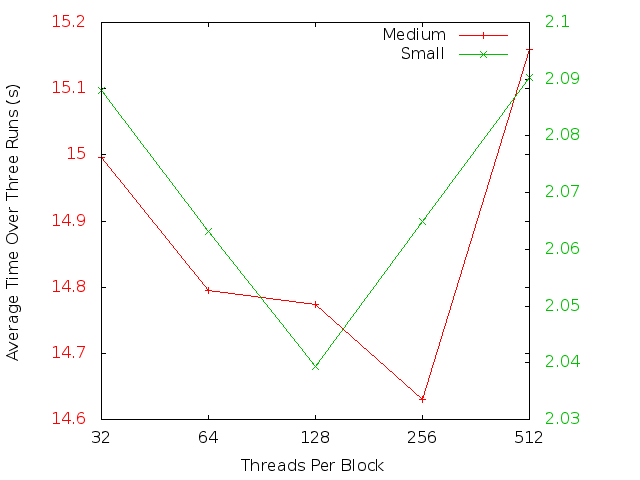
\includegraphics[scale=0.3]{images/threadsperblock}
  \caption[threadsperblock]{Threads per Block against Execution Time}
  \label{fig:threadsperblock}
\end{figure}

This shows that the optimal number of threads per block is between 64 and 256 depending upon the size of the dataset. A value of 128 seems to be a reasonable choice.

With a value of 128, we examined the occupancy value using the profiler (note that these results are with pinning disabled):

\begin{figure}[H]\centering \begin{tabular}{ l | l | l | l}
\hline
Size & Average & Min & Max \\
\hline
\hline
small & 0.429 & 0.125 & 0.500 \\
medium & 0.445 & 0.125 & 0.500 \\
\hline
\end{tabular} \end{figure}

This shows that with our sweet spot of 128 threads per block we achieve a much better occupancy than in previous tests (using a value of 32), which had an average occupancy of 0.22.